\documentclass[12pt]{article}
	\usepackage{graphicx}
	\usepackage[round]{natbib}
	\linespread{1.3}
	\bibliographystyle{plainnat}
	\title{
		Group \#07 \\
		Bridge-00 \\
		18g, 1700N \\[1cm]
		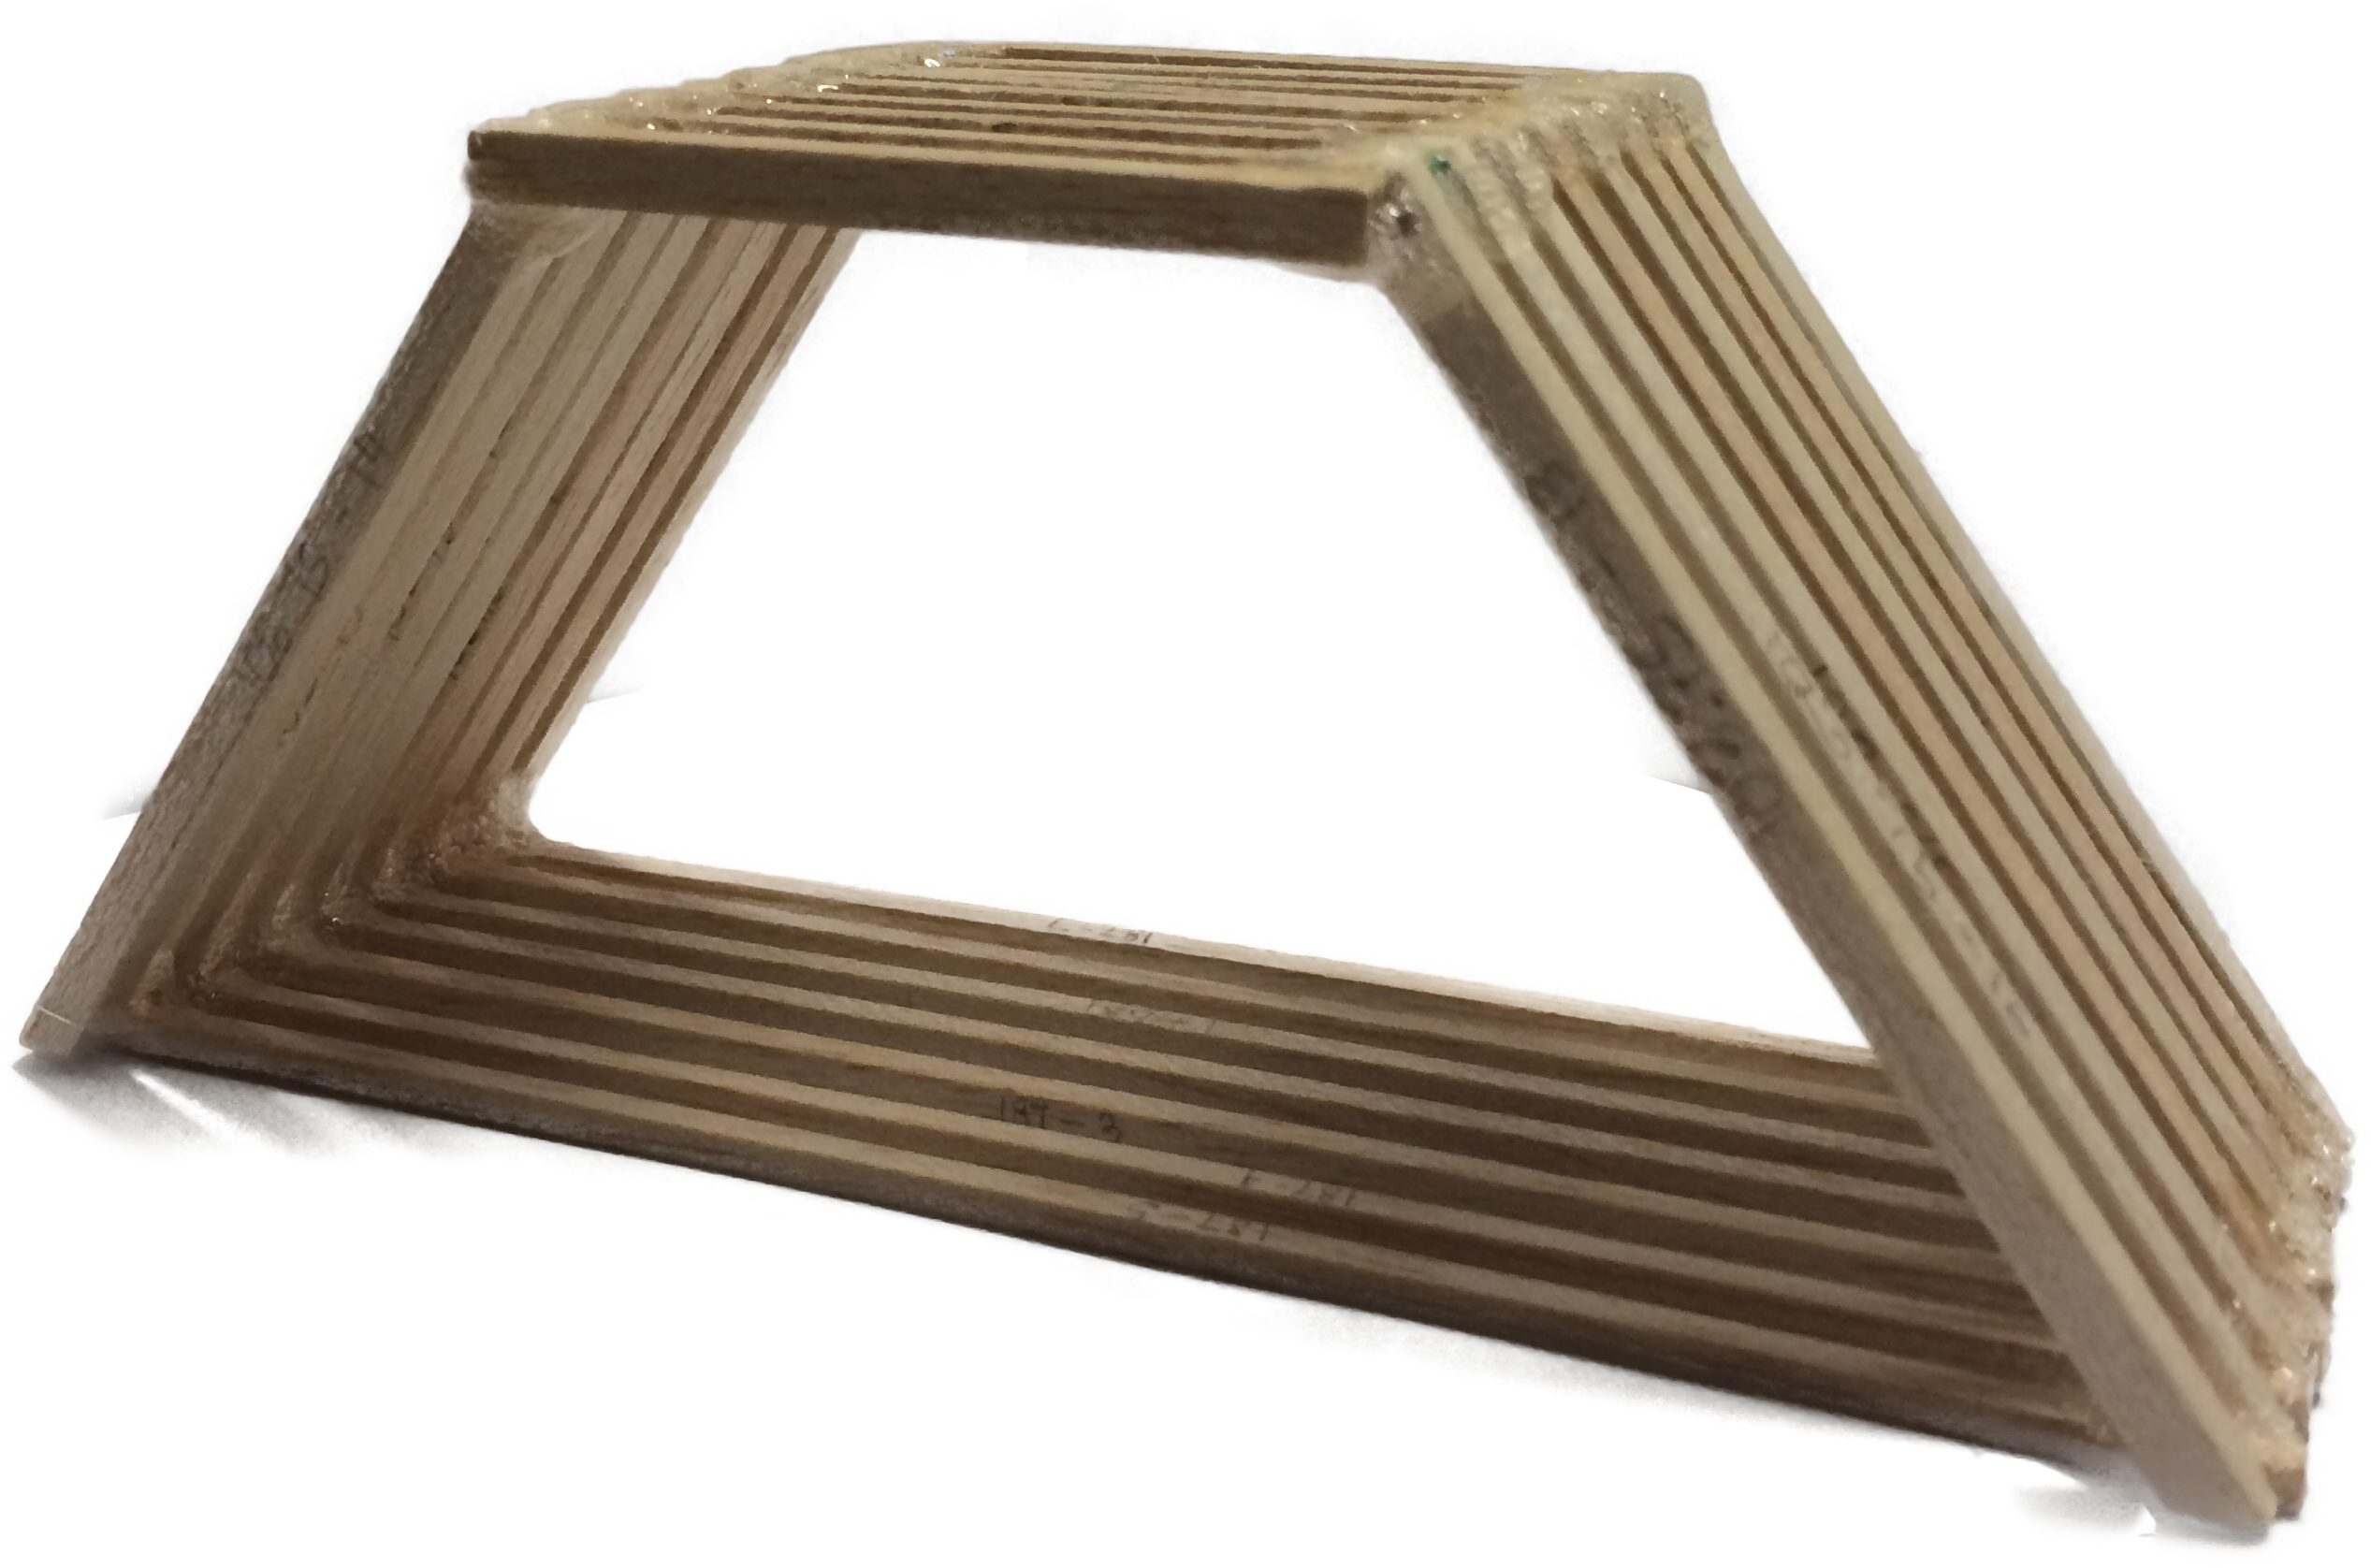
\includegraphics[width=0.7\textwidth]{photo}
	}
	\author{
		Alex Miles \\ u5568175 \\ 16.7\%
		\and Arlene Mendoza \\ u5589650 \\ 16.7\%
		\and Itsuki Nishida \\ u5578430 \\ 16.7\%
		\and Paul Apelt \\ u5568225 \\ 16.7\%
		\and Stephen Lonergan \\ u5349877 \\ 16.7\%
		\and Thomas Hale \\ u5568225 \\ 16.7\%
	}
\begin{document}
	\maketitle
	\section{Design}
		% design assumptions and methods
		\subsection{Assumptions}
		During the design process, the following assumptions have been made \citep[p.~264]{tbook}:
		\begin{enumerate}
			\item All loadings are applied at the joint,
			\item Weight of the members neglected,
			\item Joints are smooth (friction-less) pins,
			\item Each member has no more than two joints.
		\end{enumerate}
		% TODO: why trapezium
		%Talk about other designs we have considered
		%Warren truss, Pratt etc
		%Include a photo of a prototype if that is avaliable? Maybe.. Alex?
		Final bridge design can be seen in Figures \ref{dim} and \ref{proj}.
		\begin{figure}[h!]
			\centering
			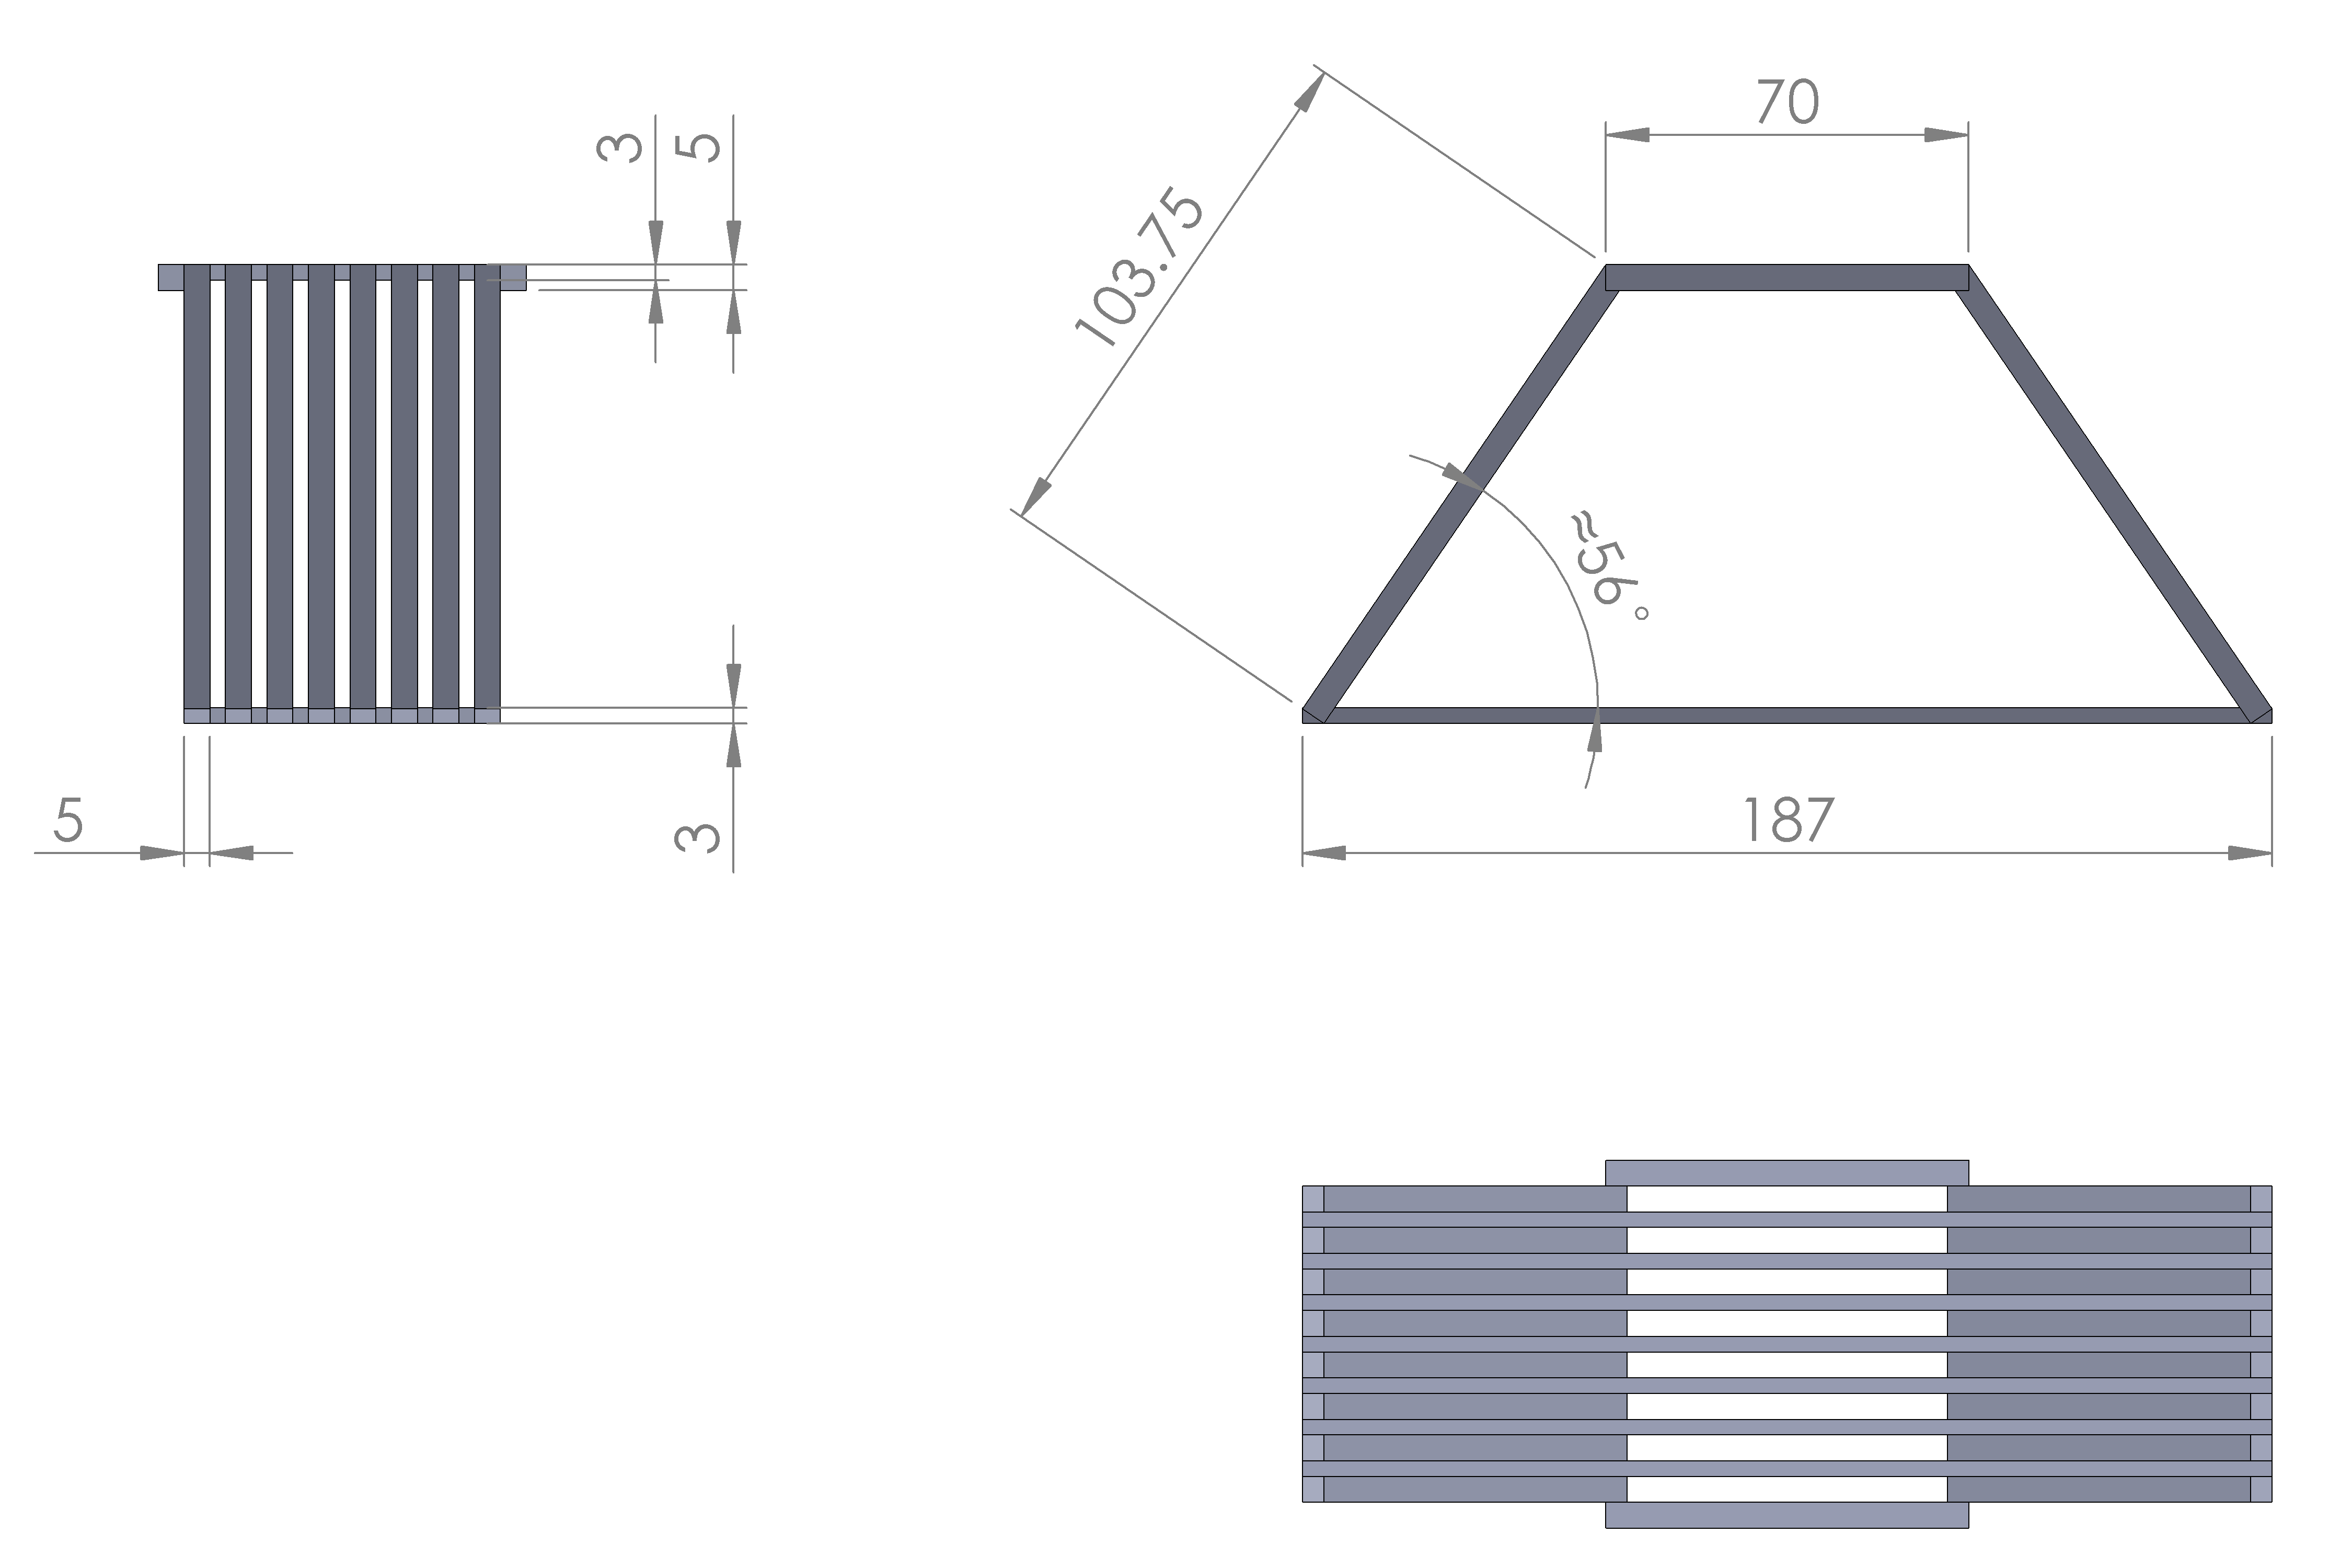
\includegraphics[width=\textwidth]{dim}
			\caption{Dimensioned drawing.}
			\label{dim}
		\end{figure}
		\begin{figure}[h!]
			\centering
			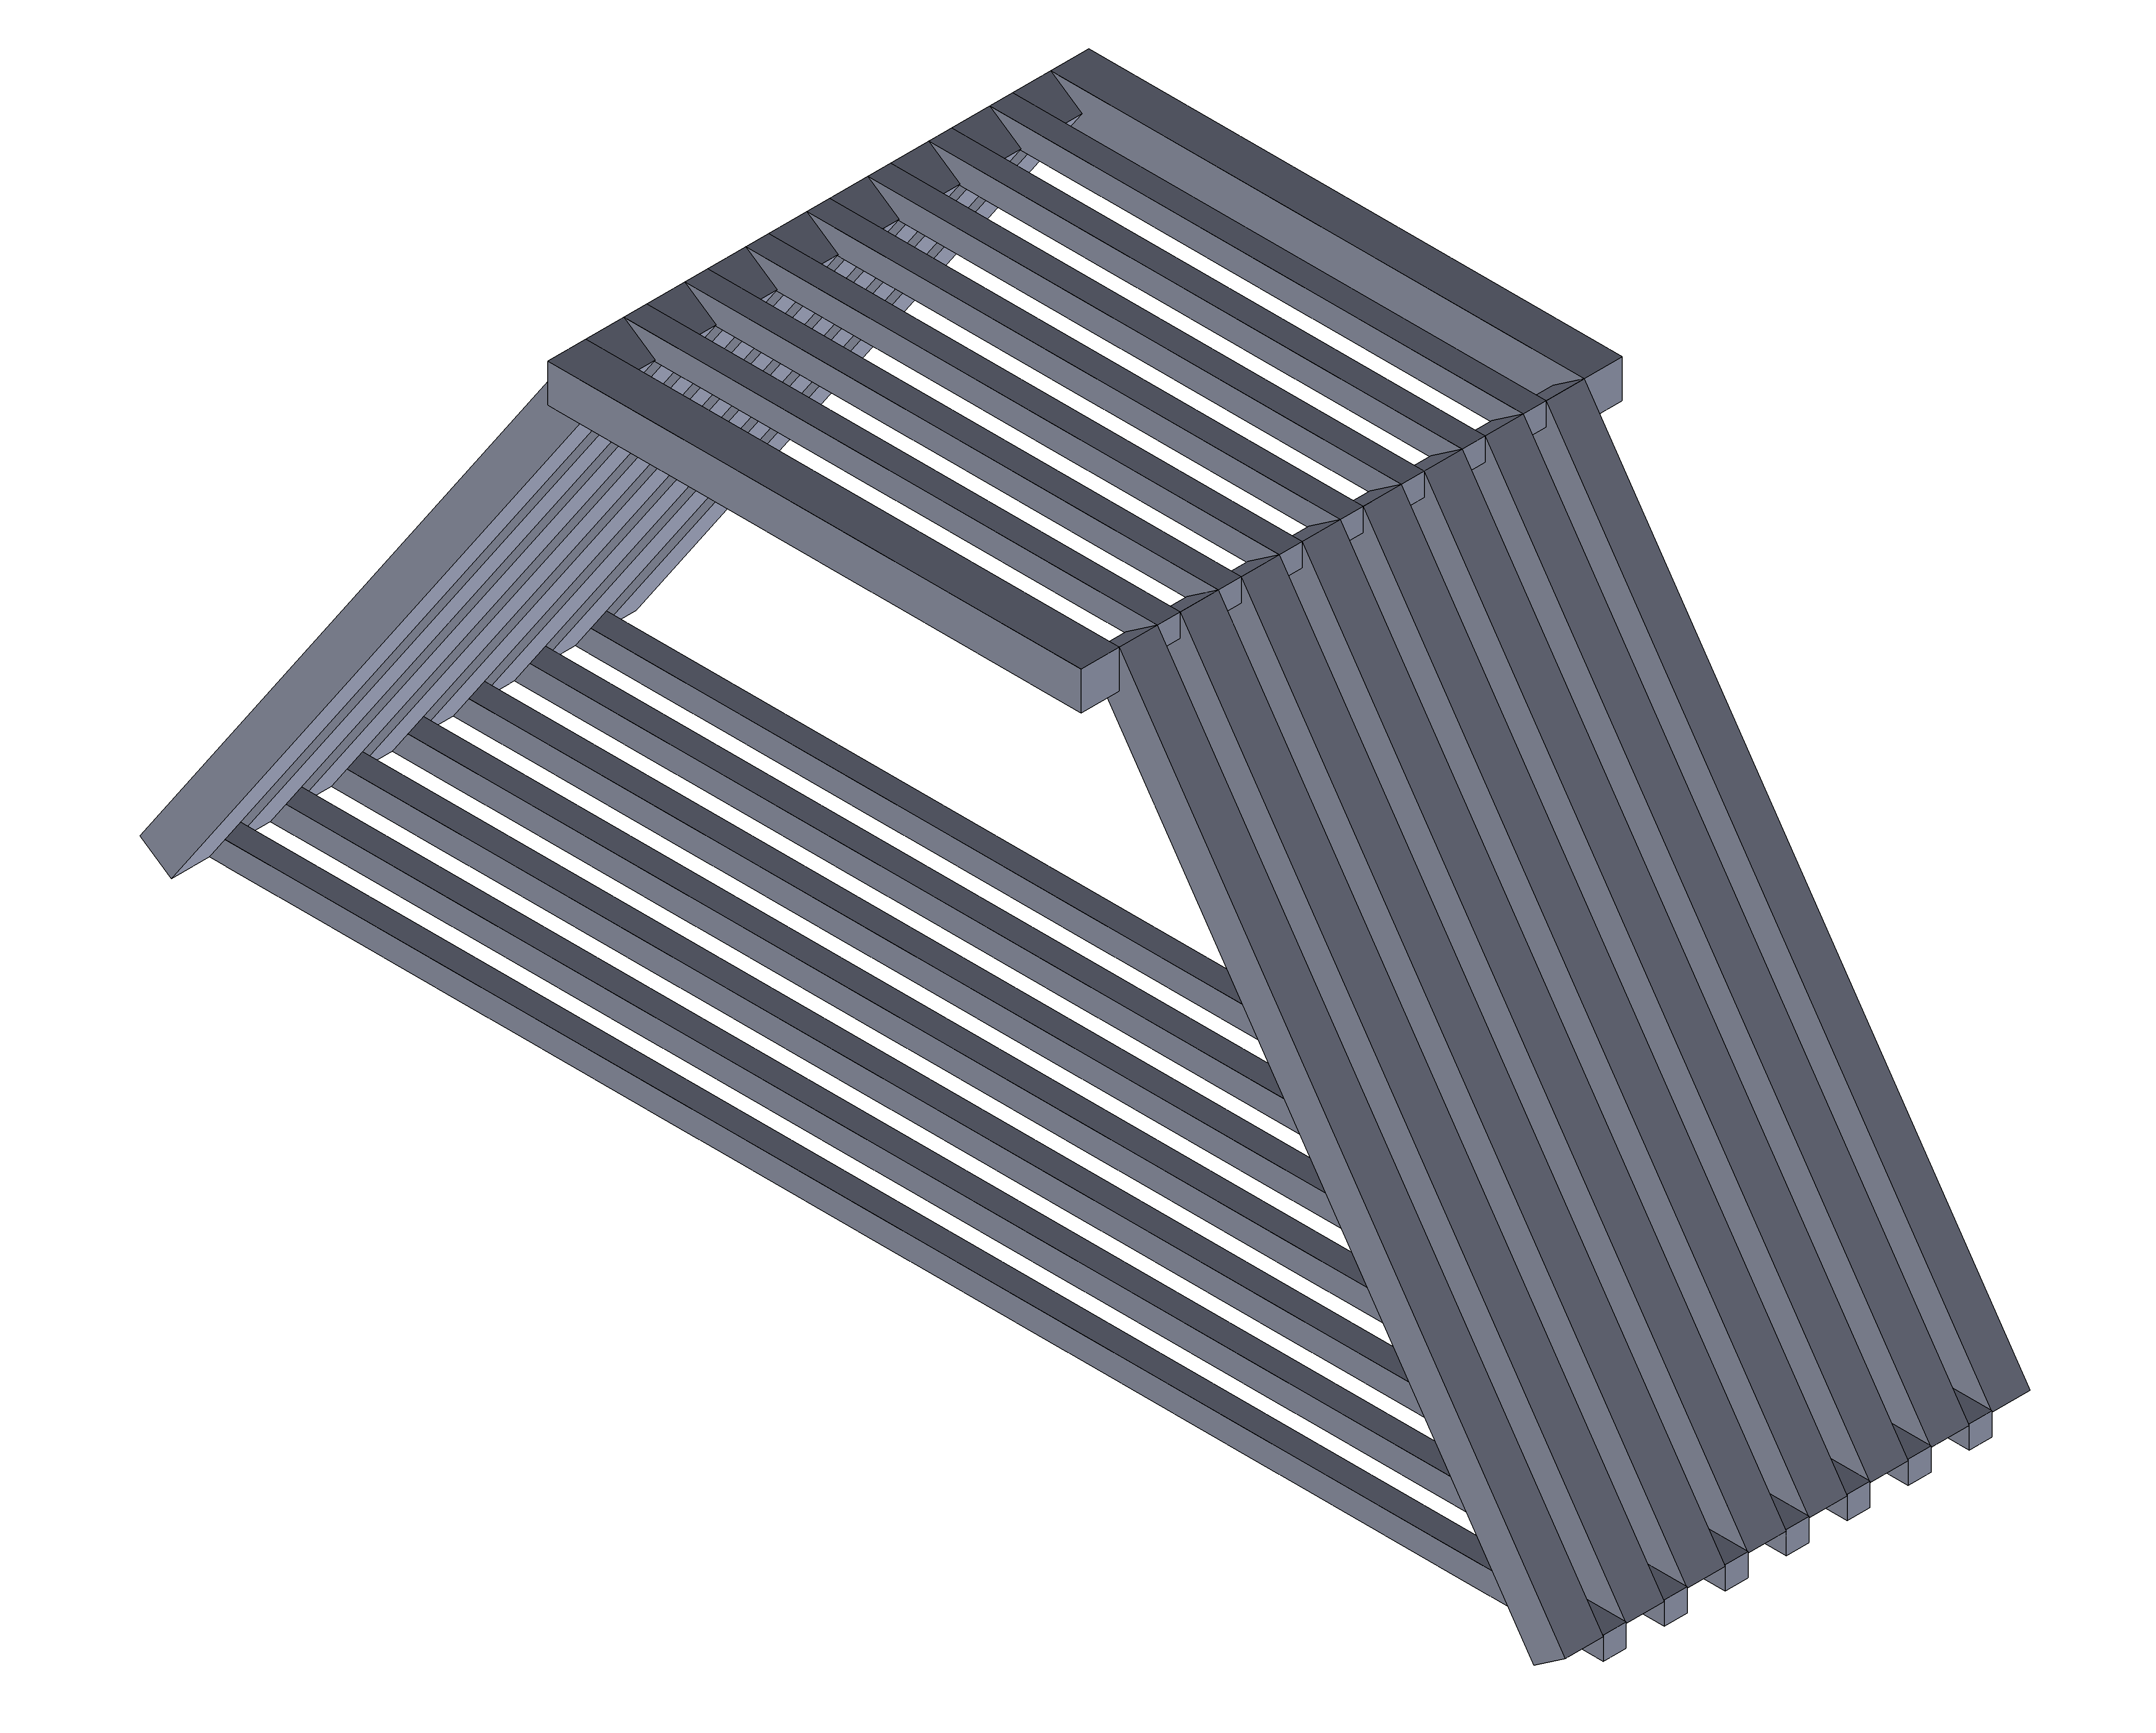
\includegraphics[width=0.6\textwidth]{proj}
			\caption{3D-Projection.}
			\label{proj}
		\end{figure}
		% dimensioned drawing
		\subsection{Methods}
		%Construction process 
		%Materials Used
		%Difficulties faced - measuring accurately, It ended up being 185mm than 187mm and the trapezium was also slightly lopsided by a 1mm
		%Weight issues - glue 
		%Insert picture of the materials used
	\section{Analysis}
		% table of member loads
		% assumptions
		% fail predictions
		% max load
		% reasons
	\section{Results}
		% analysis of the difference
		% why fail
		% much sad
		% testing machine OP
		% please nerf
	\bibliography{bib}
\end{document}

